\subsection{UC1 - Inizializzazione del sistema}
\begin{figure}[h]
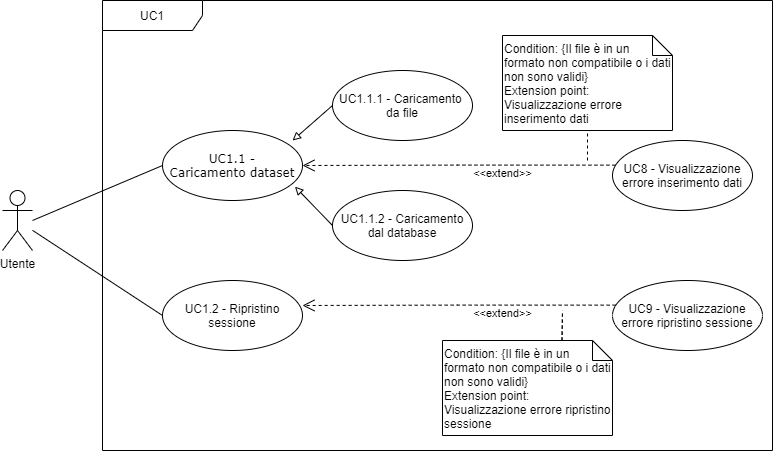
\includegraphics[width=\linewidth]{section/Images/UC1.png}
\centering
\caption{UC1 - Inizializzazione del sistema}
\end{figure}
\begin{itemize}
	\item \textbf{Attore primario}: Utente.
	\item \textbf{Precondizioni}: Il sistema è raggiungibile e funzionante.
	\item \textbf{Postcondizioni}: Viene visualizzato un messaggio che avvisa l'utente del corretto caricamento dei dati e della loro validità. I dati sono disponibili per l'analisi.
	\item \textbf{Scenario principale}:
		\begin{enumerate}
			\item L'utente accede al sistema;
			\item L'utente carica un dataset [UC1.1];
			\item L'utente, opzionalmente, seleziona un file per ripristinare una sessione di lavoro precedente [UC1.2].
			
		\end{enumerate}
	\item \textbf{Estensioni}:
	\begin{enumerate}[(a)]
		\item Nel caso in cui il file sia in un formato sbagliato o i dati non sono validi:
		\begin{enumerate}[1.]
			\item I dati non vengono caricati nel sistema;
			\item Viene visualizzato un errore esplicativo [UCxxx].
		\end{enumerate}
		
		\item Nel caso in cui il file di ripristino sessione non sia ben formattato:
		\begin{enumerate}[1.]
			\item La sessione non viene ripristinata;
			\item Viene visualizzato un errore esplicativo [UCxxx].
		\end{enumerate}
	\end{enumerate}
\end{itemize}






  